
%--------------------------------------------------------------------
\section{Incremental Behavior Modeling for Anomaly Detection}
%--------------------------------------------------------------------

\ifnum\short=0

\begin{frame}
    \frametitle{Incremental Behavior Modeling}
    \framesubtitle{Introduction}

    We propose a new \alert{incremental} method for learning behavior 
    models and detecting anomalies using HMM-based clustering on 
    a small bootstrap set of sequences labeled as normal or suspicious.
  
\end{frame}

%--------------------------------------------------------------------

\begin{frame}
    \frametitle{Incremental Behavior Modeling}
    \framesubtitle{Related Work}

    Some incremental learning approaches have been applied to 
    human behavior modeling. 

    \bigskip

    Vasquez et al.\ (2009) incrementally model vehicle and 
    pedestrian trajectories using growing hidden Markov models 
    (GHMMs). The method builds a topological map and corresponding 
    GHMM using an incremental variant of the Baum-Welch algorithm. 
    For each new node in the map, a corresponding state and 
    connectivity are added to the GHMM. 

    \bigskip 

    Kuli{\'c} and and Nakamura (2010) model movement primitives
    using HMMs and piece the primitives together with a higher 
    level HMM. Similar to Vasquez et al., the method incrementally 
    adds new hidden states when a new primitive model is built.

\end{frame}

%--------------------------------------------------------------------

\begin{frame}
    \frametitle{Incremental Behavior Modeling}
    \framesubtitle{Related Work (cont.)}

    The existing work most similar to ours is the incremental 
    learning approach of Xiang and Gong (2008), who also model 
    activity in a scene incrementally after initialization from 
    a small bootstrap dataset. 
    
    \bigskip
    
    They build explicit probabilistic models of normal and abnormal 
    activity patterns in the bootstrap set then classify new observations 
    using a likelihood ratio test. The models are global joint
    models over the entire scene. 
    
    \bigskip
    
    It is not clear how the likelihood ratio test could handle completely new
    anomalous events with low likelihoods under both models, and it 
    is not clear whether a global model is appropriate for detecting isolated 
    anomalous behavior in a scene.

\end{frame}

%--------------------------------------------------------------------

\begin{frame}
    \frametitle{Incremental Behavior Modeling}
    \framesubtitle{Overview}

    Our method does not require an a priori model of anomalous 
    human behavior. 

    \bigskip
    
    It constructs an ensemble of simple models, adding to the 
    ensemble when the existing set is insufficient to represent 
    new cases. 

    \bigskip
    
    We associate each new observation with an individual 
    model using separate statistical tests on the observation's 
    likelihood according to each individual model. 
    
\end{frame}

%--------------------------------------------------------------------

\begin{frame}
    \frametitle{Incremental Behavior Modeling}
    \framesubtitle{Overview (cont.)}
    
    Rather than globally modeling the entire scene, our method 
    takes a more local approach, separately analyzing each individual 
    moving object's behavior. 

    \bigskip
    
    In an experimental comparison of the two methods, we find 
    \begin{itemize}
        \item {\em statistical testing of the likelihood} is superior to 
            {\em likelihood ratio tests}; 
        \item {\em local representation} is superior to {\em global 
            representation}.
    \end{itemize}

\end{frame}

%--------------------------------------------------------------------

\begin{frame}
    \frametitle{Incremental Behavior Modeling}
    \framesubtitle{Overview (cont.)}
    
    After bootstrapping, we assign new observation sequences to 
    behavior clusters using statistical tests on the log likelihood 
    of the sequence according to the corresponding HMMs.

    \bigskip

    We label a sequence as suspicious if it maps to an existing 
    model of suspicious behavior or does not map to any existing 
    model. 

    \bigskip

    After labeling, we either incrementally update the sufficient 
    statistics for the most likely HMM's parameters or create a new 
    HMM for the new sequence.

\end{frame}

%--------------------------------------------------------------------

\begin{frame}
    \frametitle{Incremental Behavior Modeling}
    \framesubtitle{Contribution}

    The main contribution is a new modeling method for 
    \begin{itemize}
        \item detection of anomalous events in 
            surveillance video based on simply-structured models; 
        \item incremental learning that is demonstrably able to evolve 
            the models over time to adapt to new behavior and also
            outperforms current techniques on the same data set.
    \end{itemize}

\end{frame}

%--------------------------------------------------------------------

\begin{frame}
    \frametitle{Incremental Behavior Modeling}
    \framesubtitle{Methodology}

    Methods that are involved in this work:
    \begin{itemize}
        \item Blob extraction and tracking from ``Blob-Based Motion Anlaysis''
        \item Behavior model bootstrapping from ``Clustering Human Behaviors''
        \item Anomaly Detection from ``Detection from a Small Bootstrap Set''
        \item Incremental Behavior Modeling
    \end{itemize}

\end{frame}

%--------------------------------------------------------------------

\begin{frame}
    \frametitle{Incremental Behavior Modeling}
    \framesubtitle{Pseudocode for Anomaly Detection with 
        Incremental Learning}

    \begin{algorithm}[H]
        \caption{Anomaly Detection with Incremental Learning}
        \label{anomaly-detection-with-iml-algorithm}
        \begin{algorithmic}
            \REQUIRE $\vec{O}$: behavior sequence 
            \REQUIRE ${\cal M}$: set of HMMs 
            \REQUIRE ${\cal S}$: set of sufficient statistics 
            \ENSURE $\widetilde{\cal M}$: set of revised HMMs 
            \ENSURE $\widetilde{\cal S}$: set of revised sufficient statistics

            \STATE $\widetilde{\cal M} \gets {\cal M}; \; \widetilde{\cal S} \gets {\cal S}$
            \STATE ${\cal M}_{ab} \gets \{ M \mid M \in {\cal M} \text{~and $M$ is marked abnormal} \}$ 

            \STATE $( M_{ml}, S_{ml}, L_{ml} ) \gets
                \textsc{Find-Most-Likely-Model}(\vec{O}, {\cal M})$ 
            \STATE $d_{\text{feedback}} \gets \emptyset$

            \IF{$M_{ml} \in {\cal M}_{ab}$ or $L_{ml} \leq \theta_z$}
                \STATE $d_{\text{feedback}} \gets \textsc{Alert-Security-Personnel}(\vec{O})$
            \ENDIF

            \algstore{iml}

        \end{algorithmic}
    \end{algorithm}

\end{frame}

%--------------------------------------------------------------------

\begin{frame}
    \frametitle{Incremental Behavior Modeling}
    \framesubtitle{Pseudocode for Anomaly Detection with 
        Incremental Learning (cont.)}

    \begin{algorithm}[H]
        \begin{algorithmic}
            \algrestore{iml}
        
            \IF{$L_{ml} > \theta_z$ and $d_{\text{feedback}} \neq$ false positive} 
                \STATE $( M, S ) \gets \textsc{Incrementally-Update}(M_{ml}, S_{ml})$ 
                \STATE $\widetilde{\cal M} \gets \{ \widetilde{\cal
                    M}\;$\textbackslash$\;M_{ml} \} \cup \{ M \}; \; \widetilde{\cal S} \gets \{ \widetilde{\cal
                    S}\;$\textbackslash$\;S_{ml} \} \cup \{ S \}$ 
            \ELSE 
                \STATE $( M, S ) \gets \textsc{Create-New-Model}(\vec{O})$

                \IF{$L_{ml} \le \theta_z$ and $d_{\text{feedback}} \neq$ false positive} 
                    \STATE Mark $M$ as abnormal 
                \ENDIF

                \STATE $\widetilde{\cal M} \gets \widetilde{\cal M} \cup \{ M \}; \; \widetilde{\cal S} \gets \widetilde{\cal S} \cup \{ S \}$ 
            \ENDIF
        \end{algorithmic}
    \end{algorithm}

\end{frame}

%--------------------------------------------------------------------

\begin{frame}
    \frametitle{Incremental Behavior Modeling}
    \framesubtitle{Pseudocode for Incremental Learning}

    \begin{algorithm}[H]
        \caption{Incremental EM Algorithm}
        \label{incremental-em-algorithm}
        \begin{algorithmic}
            \REQUIRE $\vec{O}$: behavior sequence
            \REQUIRE $M$: HMM model
            \REQUIRE ${\cal S} = \{ \vec{\Gamma}, \vec{\Xi} \}$: set of sufficient statistics
            \ENSURE $M^*$: revised HMM model
            \ENSURE ${\cal S}^* = \{ \vec{\Gamma}^*, \vec{\Xi}^* \}$: set of revised sufficient statistics
            \STATE $M^* \gets M$
            \FOR{$i = 1 \to I$}
                \STATE \COMMENT{E-step}
                \STATE $(\vec{\gamma}, \vec{\xi}) \gets \textsc{Compute-Sufficient-Statistics}(\vec{O}, M^*)$
                \STATE $\vec{\Gamma}^* \gets \alpha \vec{\Gamma} + \vec{\gamma}$; \; $\vec{\Xi}^* \gets \alpha \vec{\Xi} + \vec{\xi}$
                \STATE \COMMENT{M-step}
                \STATE $M^* \gets \textsc{Reestimate-Model-Parameters}(M^*, \vec{\Gamma}^*, \vec{\Xi}^*)$
            \ENDFOR
        \end{algorithmic}
    \end{algorithm}

\end{frame}

%--------------------------------------------------------------------

\begin{frame}
    \frametitle{Incremental Behavior Modeling}
    \framesubtitle{Experimental Results}

    We performed experiments in three parts:
    \begin{enumerate}
        \item model configuration selection (finding an optimal 
            set of HMMs to model the bootstrap set); 
        \item anomaly detection based on the HMM bootstrap set; 
        \item anomaly detection with incrementl learning.
    \end{enumerate}

\end{frame}

%--------------------------------------------------------------------

\begin{frame}
    \frametitle{Incremental Behavior Modeling}
    \framesubtitle{Experimental Results (cont.)}

    In model configuration selection experiment
    \begin{itemize}
        \item Performed five-fold cross validation with different 
            bootstrap parameter settings; 
        \item Selected the configuration with the highest accuracy 
            in separating the normal sequences from the abnormal 
            sequences on the bootstrap set, as measured by the 
            \alert{false positive rate} for abnormal sequences over 
            all cross validation test folds. 
    \end{itemize}

    Every bootstrap cluster containing an abnormal sequence is considered 
    abnormal, so we always obtain 100\% detection on the bootstrap set;
    the only discriminating factor is the false positive rate.

\end{frame}

%--------------------------------------------------------------------

\begin{frame}
    \frametitle{Incremental Behavior Modeling}
    \framesubtitle{Experimental Results (cont.)}

    In the anomaly detection (batch processing) experiment, we compare 
    the proposed method against HMM-based methods using alternative 
    representations and scoring methods similar to those of Xiang and 
    Gong (2008).

    \medskip

    \begin{block}{Different Event Representations}
        Local representation vs.\ Xiang and Gong's global 
        representation
    \end{block}
    
    \begin{block}{Different Scoring Methods}
        $z$-scoring method vs.\ the standard likelihood ratio 
        test (LRT)
    \end{block}


\end{frame}

%--------------------------------------------------------------------

\begin{frame}
    \frametitle{Incremental Behavior Modeling}
    \framesubtitle{Experimental Results (cont.)}
    
    The four methods are as follows:
    \begin{enumerate}
        \item {\bf Method I:} The proposed method.
        \item {\bf Method II:} The proposed method, but using Xiang and Gong's
            likelihood ratio test (Xiang and Gong, 2008)
            rather than our $z$-scored likelihood method.
        \item {\bf Method III:} An HMM-based method using a global event
            representation similar to that of Xiang and Gong, with our
            $z$-scored likelihood method.
        \item {\bf Method IV:} The global method (Method III) using Xiang and
            Gong's likelihood ratio test rather than our $z$-scored likelihood
            method.
    \end{enumerate}

\end{frame}

%--------------------------------------------------------------------

\begin{frame}
    \frametitle{Incremental Behavior Modeling}
    \framesubtitle{Experimental Results (cont.)}
    
    \begin{table}
        \caption{Example human behavior pattern bootstrapping
            results. We used linear HMMs with five states and seven
            symbols. The model consists of 17 clusters. ``W'' means ``walk''
            and ``C'' means ``cycle.'' For the six clusters containing more
            than one sequence, shown is the distribution of the patterns in
            the cluster over the activities.  The last row shows the
            distribution of the 11 clusters containing only a single sequence
            over the activity categories.}
        \centering
        \begin{tabular}{c|c|c|c|c|c}
            \hline
            Cluster \# & W-in & W-out & C-in & C-out & Other \\
            \hline \hline
            1 & 44 & 0  & 20 & 0  & 0 \\ \hline
            2 & 0  & 38 & 0  & 24 & 0 \\ \hline
            3 & 0  & 0  & 3  & 0  & 0 \\ \hline
            4 & 0  & 0  & 2  & 0  & 0 \\ \hline
            5 & 0  & 0  & 0  & 0  & 6 \\ \hline
            6 & 0  & 0  & 0  & 0  & 2 \\ \hline
            One-seq clusters & 0 & 1 & 6 & 1 & 3 \\ \hline
        \end{tabular}
        \label{tab:bootstrapping-results}
    \end{table}

\end{frame}

%--------------------------------------------------------------------

\begin{frame}
    \frametitle{Incremental Behavior Modeling}
    \framesubtitle{Experimental Results (cont.)}
    
    \begin{figure}
        \centering
        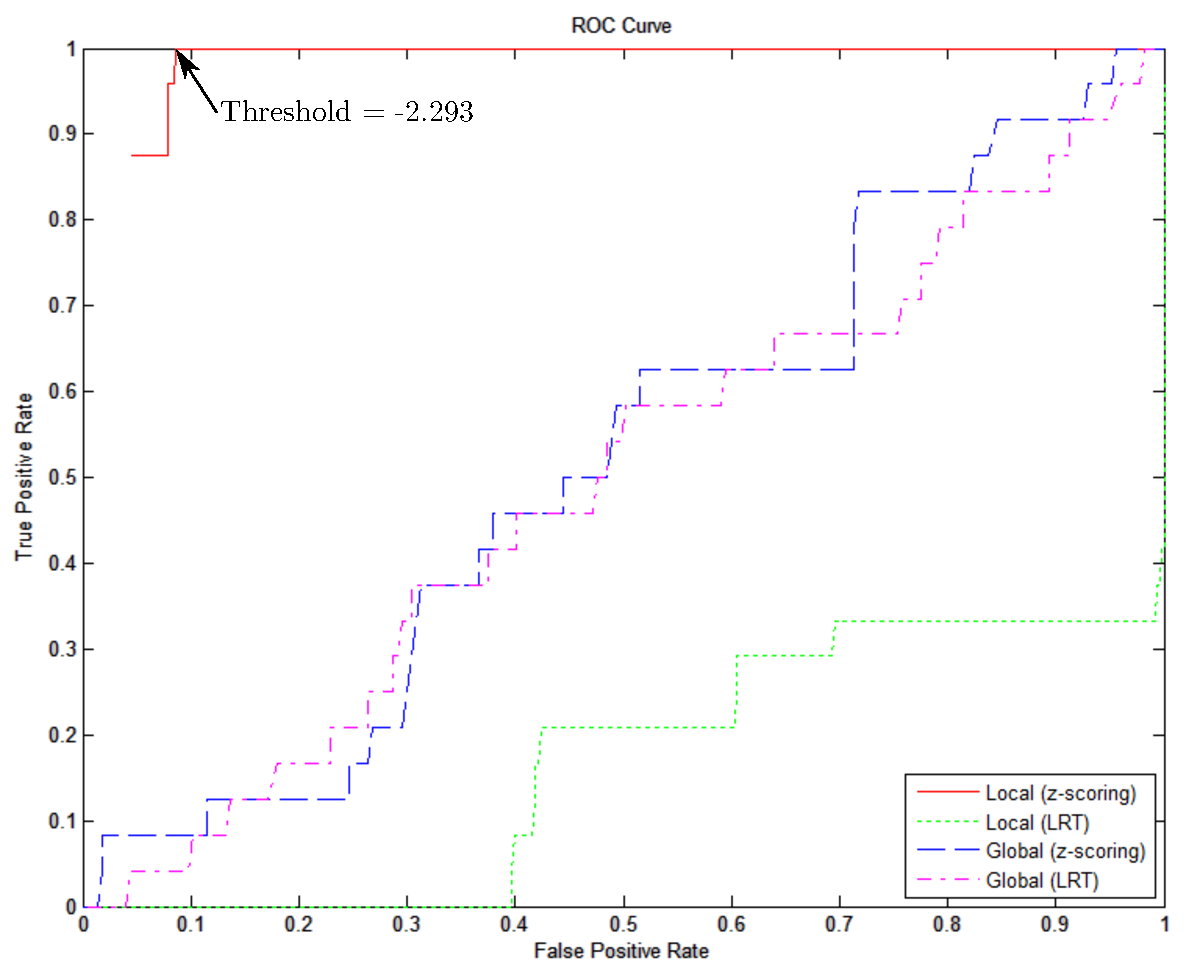
\includegraphics[width=2.8in]{figures/roc-ours-vs-global-results}
        \caption{Anomaly detection ROC
            curves. Solid red, dotted green, dashed blue, and dash-dot magenta
            lines represent ROCs for methods I, II, III, and IV,
            respectively.}
        \label{fig:roc-ours-vs-global-results}
    \end{figure}

\end{frame}

%--------------------------------------------------------------------

\begin{frame}
    \frametitle{Incremental Behavior Modeling}
    \framesubtitle{Experimental Results (cont.)}
    
    The ROC curves and FP rates show that our method clearly outperforms
    the other three methods, but there is also a surprising interaction.

    \bigskip

    For the global method, $z$-scored likelihood and LRT are equally
    effective, but for our local event based method, $z$-scoring is much
    more effective than the LRT.  
    
    \bigskip
    
    This may reflect that the LRT's use of a mixture model is less 
    appropriate for the local method than the global method.
    
\end{frame}

%--------------------------------------------------------------------

\begin{frame}
    \frametitle{Incremental Behavior Modeling}
    \framesubtitle{Experimental Results (cont.)}
    
    \begin{table}
        \centering
        \caption{Anomaly detection results for the local method with
            the $z$-scoring method and the likelihood ratio test, and the
            global method with the $z$-scoring method and likelihood ratio
            test.}
        \begin{tabular}{c|c|c|c|c|c|c}
            \hline Batch method & TP & FP & TN & FN & TPR & FPR \\ \hline \hline
            Local ($z$-scoring) & 24 & 42 & 444 & 0 & 1 & 0.086 \\ \hline
            Local (LRT) & 24 & 486 & 0 & 0 & 1 & 1 \\ \hline 
            Global ($z$-scoring) & 24 & 217 & 10 & 0 & 1 & 0.956 \\ \hline 
            Global (LRT) & 24 & 223 & 4 & 0 & 1 & 0.982 \\ \hline
        \end{tabular}
        \label{tab:hmm-based-detection-results}
    \end{table} 

\end{frame}

%--------------------------------------------------------------------

\begin{frame}
    \frametitle{Incremental Behavior Modeling}
    \framesubtitle{Experimental Results (cont.)}
    
    The reason that the local method is better than the global method
    (albeit when combined with $z$-scoring of the likelihood) is that 
    
    \begin{itemize}
        \item Many of the abnormal sequences in the test set tend to be 
            locally similar to the abnormal sequences in the bootstrap set 
            but globally different. 
        \item The local method treats concurrent but spatially separate
            local events as being independent, whereas the global method 
            attempts to construct a joint model over the entire scene. 
            The global method might be improved with a larger bootstrap set.
    \end{itemize}

\end{frame}

%--------------------------------------------------------------------

\begin{frame}
    \frametitle{Incremental Behavior Modeling}
    \framesubtitle{Experimental Results (cont.)}
    
    The log likelihood ratio test fails to detect completely new anomalous
    patterns when the pattern has a very low likelihood according to the
    abnormal model and the normal model but has a slightly higher
    likelihood according to the normal model. 
    
    \bigskip
    
    In order for the LRT test to
    detect such patterns, we need to adjust the LR threshold, causing
    higher false positives (increasing the number of false positives to
    about 30--40).  
    
    \bigskip
    
    Since our approach creates a new abnormal model for
    any low-likelihood observation, regardless of the relative likelihood,
    it does not suffer from this problem.
    
\end{frame}

%--------------------------------------------------------------------

\begin{frame}
    \frametitle{Incremental Behavior Modeling}
    \framesubtitle{Experimental Results (cont.)}
    
    We used the same settings and model configuration as in the batch 
    method experiments.
   
    \bigskip

    Since we incorporate a completely new observation sequence at each 
    increment, the likelihood over all the sequences may increase or 
    decrease. 
    
    \bigskip
    
    In the current work, we reestimate $\mu_c$ and $\sigma_c$ after every 
    update by generating 1,000 new sample sequences.  The update process 
    could obviously be optimized.

\end{frame}

%--------------------------------------------------------------------

\begin{frame}
    \frametitle{Incremental Behavior Modeling}
    \framesubtitle{Experimental Results (cont.)}

    To further understand the performance differences between the batch
    and incremental methods, we partitioned the test data sequentially
    into chunks and computed the false and true positive rates for each
    chunk of observations.  
    
\end{frame}



%--------------------------------------------------------------------

\begin{frame}
    \frametitle{Incremental Behavior Modeling}
    \framesubtitle{Experimental Results (cont.)}

    \begin{figure}
        \centering
        \subfloat[]{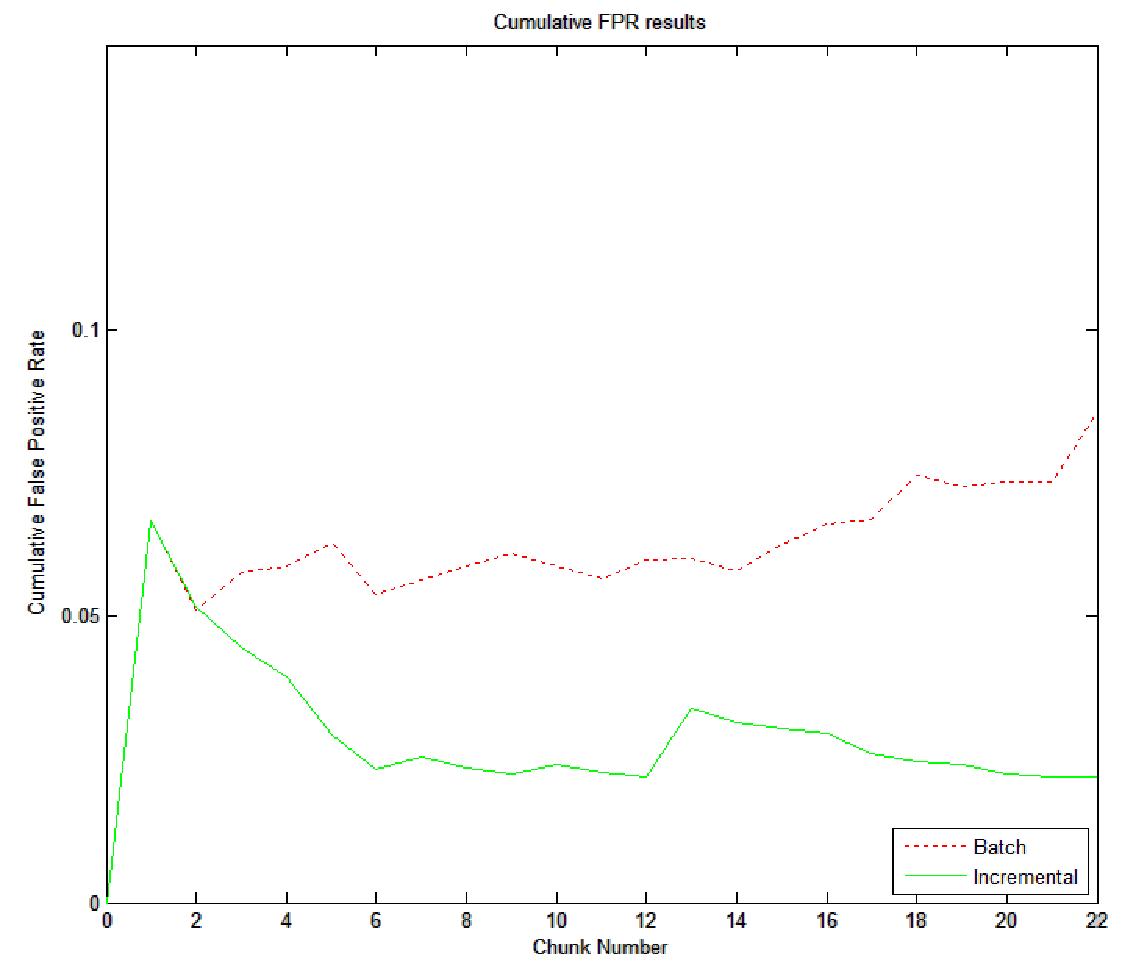
\includegraphics[width=2.2in]{figures/cFPR-chunk-results-5-trials}}
        \subfloat[]{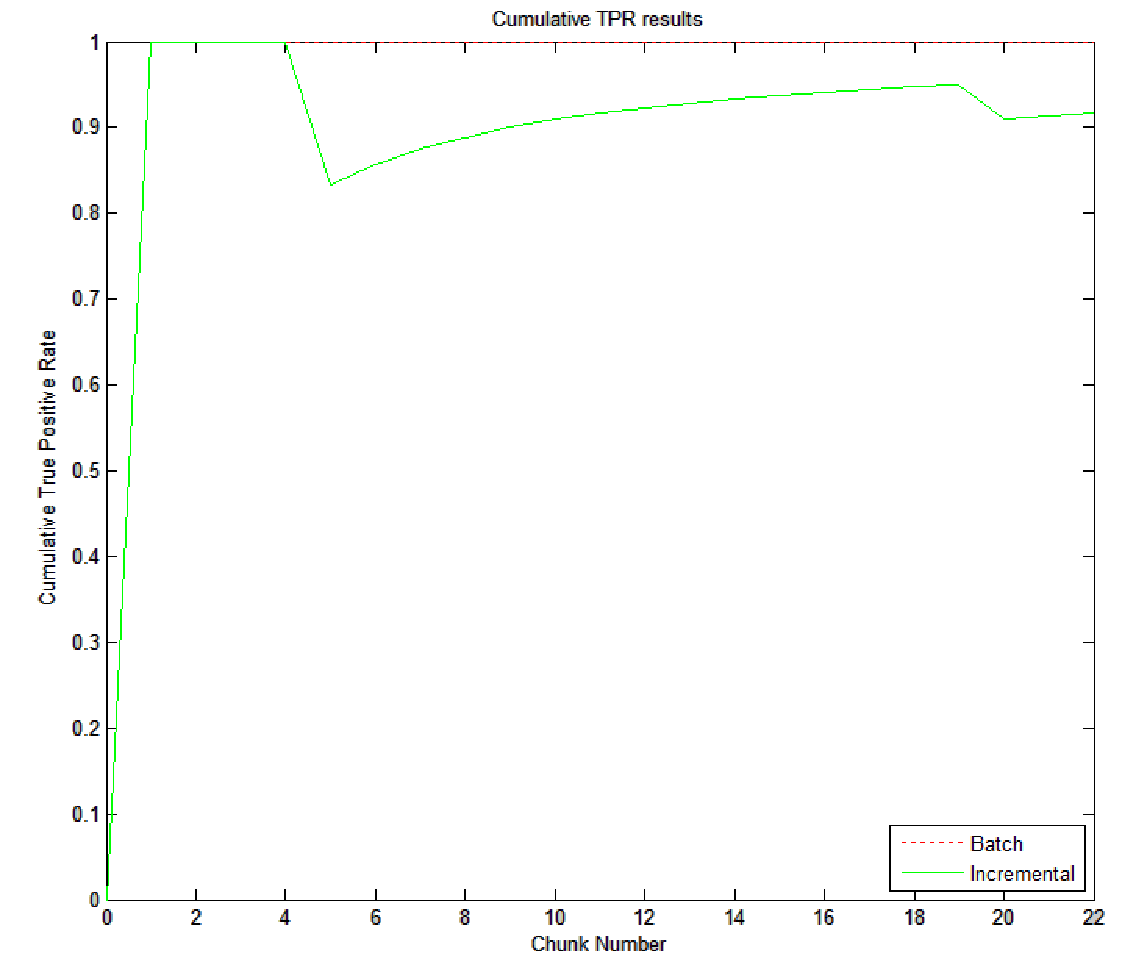
\includegraphics[width=2.2in]{figures/cTPR-chunk-results-5-trials}}
        \caption{Comparison of batch learning (dotted red line) and
            incremental learning (solid green line) over time.  (a) Cumulative
            false positive rates. (b) Cumulative true positive rates.  Each
            point is an average of the false positive or true positive rates
            over 5 trials.}
        \label{fig:chunking-results}
    \end{figure}

\end{frame}

%--------------------------------------------------------------------

\begin{frame}
    \frametitle{Incremental Behavior Modeling}
    \framesubtitle{Experimental Results (cont.)}

    \begin{table}
        \caption{Anomaly detection results on average for
            incremental HMM learning for our local method and the global
            method over 5 trials.}
            \centering
            \begin{tabular}{c|c|c|c|c|c|c}
                \hline
                Incremental method & TP & FP & TN & FN & TPR & FPR \\
                \hline \hline
                Local ($z$-scoring) & 21.8 & 9.8  & 476.2  & 2.2 & 0.91 & 0.022 \\ \hline
                Local (LRT) & 16 & 243.4 & 212.6 & 8 & 0.6664 & 0.564 \\ \hline
                Global ($z$-scoring)  & 3 & 13 & 214 & 21 & 0.125 & 0.057 \\ \hline
                Global (LRT)  & 18 & 184.4 & 42.6 & 6 & 0.75 & 0.813 \\ \hline
            \end{tabular}
        \label{tab:iml-detection-results}
    \end{table}

\end{frame}

%--------------------------------------------------------------------

\begin{frame}
    \frametitle{Incremental Behavior Modeling}
    \framesubtitle{Experimental Results (cont.)}

    Compared to the batch method, the
    incremental version of the proposed method (local method with
    $z$-scoring) obtains a nearly four-fold decrease in the false positive
    rate (2.2\% vs.\ 8.6\%) at the cost of a 9\% decrease in the hit rate.

    \bigskip
    
    To better enable comparison of the
    results for batch and incremental learning, we varied $\theta_z$ to
    obtain false positive rates at 100\% detection rates and to obtain
    equal error rates (EERs). 
    
    \bigskip
    
    The incremental method achieves a 3.7\%
    false alarm rate at a 100\% hit rate, compared to 8.6\% for the batch
    method.  It achieves an EER of 95.8\%, compared to 91.8\% for the
    batch method.

\end{frame}

%--------------------------------------------------------------------

\begin{frame}
    \frametitle{Incremental Behavior Modeling}
    \framesubtitle{Discussion}

    We have proposed an efficient method for bootstrapping 
    scene-specific anomalous human behavior detection systems that 
    incrementally learns behavior models \alert{without} requiring storage
    of large databases of training data. 
    
    \bigskip
    
    The method requires minimal involvement of a human operator; the only 
    required action is to label the 
    patterns in a small bootstrap set as normal or anomalous and
    then to label false positive alarms as normal when they occur.

\end{frame}

%--------------------------------------------------------------------

\begin{frame}
    \frametitle{Incremental Behavior Modeling}
    \framesubtitle{Discussion (cont.)}

    On a testbed data set acquired in a real-world video surveillance 
    situation, with a bootstrap set of 
    150 sequences, the incremental method achieves a false positive rate of 
    2.2\% at a 91\% hit rate. With
    threshold tuning, the method can yield an equal error rate of 95.8\% 
    or a false positive rate of 3.7\% at a 100\% hit rate. 
    
    \bigskip
    
    The experiments show that it is possible to learn a complex 
    set of varied behaviors occurring in a specific scene with a collection 
    of simple HMMs while allowing evolution of the
    learned typical behavior model over time. This can lead in turn to more 
    effective anomaly detection.

\end{frame}

%--------------------------------------------------------------------

\else

\begin{frame}
    \frametitle{Incremental Behavior Modeling}
    \framesubtitle{Introduction}

    The main contribution is a new modeling method for 
    \begin{itemize}
        \item detection of anomalous events in 
            surveillance video based on simply-structured models; 
        \item incremental learning that is demonstrably able to evolve 
            the models over time to adapt to new behavior and also
            outperforms current techniques on the same data set.
    \end{itemize}

\end{frame}

%--------------------------------------------------------------------

\begin{frame}
    \frametitle{Incremental Behavior Modeling}
    \framesubtitle{Pseudocode for Anomaly Detection with 
        Incremental Learning}

    \begin{algorithm}[H]
        \caption{Anomaly Detection with Incremental Learning}
        \label{anomaly-detection-with-iml-algorithm}
        \begin{algorithmic}
            \REQUIRE $\vec{O}$: behavior sequence 
            \REQUIRE ${\cal M}$: set of HMMs 
            \REQUIRE ${\cal S}$: set of sufficient statistics 
            \ENSURE $\widetilde{\cal M}$: set of revised HMMs 
            \ENSURE $\widetilde{\cal S}$: set of revised sufficient statistics

            \STATE $\widetilde{\cal M} \gets {\cal M}; \; \widetilde{\cal S} \gets {\cal S}$
            \STATE ${\cal M}_{ab} \gets \{ M \mid M \in {\cal M} \text{~and $M$ is marked abnormal} \}$ 

            \STATE $( M_{ml}, S_{ml}, L_{ml} ) \gets
                \textsc{Find-Most-Likely-Model}(\vec{O}, {\cal M})$ 
            \STATE $d_{\text{feedback}} \gets \emptyset$

            \IF{$M_{ml} \in {\cal M}_{ab}$ or $L_{ml} \leq \theta_z$}
                \STATE $d_{\text{feedback}} \gets \textsc{Alert-Security-Personnel}(\vec{O})$
            \ENDIF

            \algstore{iml}

        \end{algorithmic}
    \end{algorithm}

\end{frame}

%--------------------------------------------------------------------

\begin{frame}
    \frametitle{Incremental Behavior Modeling}
    \framesubtitle{Pseudocode for Anomaly Detection with 
        Incremental Learning (cont.)}

    \begin{algorithm}[H]
        \begin{algorithmic}
            \algrestore{iml}
        
            \IF{$L_{ml} > \theta_z$ and $d_{\text{feedback}} \neq$ false positive} 
                \STATE $( M, S ) \gets \textsc{Incrementally-Update}(M_{ml}, S_{ml})$ 
                \STATE $\widetilde{\cal M} \gets \{ \widetilde{\cal
                    M}\;$\textbackslash$\;M_{ml} \} \cup \{ M \}; \; \widetilde{\cal S} \gets \{ \widetilde{\cal
                    S}\;$\textbackslash$\;S_{ml} \} \cup \{ S \}$ 
            \ELSE 
                \STATE $( M, S ) \gets \textsc{Create-New-Model}(\vec{O})$

                \IF{$L_{ml} \le \theta_z$ and $d_{\text{feedback}} \neq$ false positive} 
                    \STATE Mark $M$ as abnormal 
                \ENDIF

                \STATE $\widetilde{\cal M} \gets \widetilde{\cal M} \cup \{ M \}; \; \widetilde{\cal S} \gets \widetilde{\cal S} \cup \{ S \}$ 
            \ENDIF
        \end{algorithmic}
    \end{algorithm}

\end{frame}

%--------------------------------------------------------------------

\begin{frame}
    \frametitle{Incremental Behavior Modeling}
    \framesubtitle{Pseudocode for Incremental Learning}

    \begin{algorithm}[H]
        \caption{Incremental EM Algorithm}
        \label{incremental-em-algorithm}
        \begin{algorithmic}
            \REQUIRE $\vec{O}$: behavior sequence
            \REQUIRE $M$: HMM model
            \REQUIRE ${\cal S} = \{ \vec{\Gamma}, \vec{\Xi} \}$: set of sufficient statistics
            \ENSURE $M^*$: revised HMM model
            \ENSURE ${\cal S}^* = \{ \vec{\Gamma}^*, \vec{\Xi}^* \}$: set of revised sufficient statistics
            \STATE $M^* \gets M$
            \FOR{$i = 1 \to I$}
                \STATE \COMMENT{E-step}
                \STATE $(\vec{\gamma}, \vec{\xi}) \gets \textsc{Compute-Sufficient-Statistics}(\vec{O}, M^*)$
                \STATE $\vec{\Gamma}^* \gets \alpha \vec{\Gamma} + \vec{\gamma}$; \; $\vec{\Xi}^* \gets \alpha \vec{\Xi} + \vec{\xi}$
                \STATE \COMMENT{M-step}
                \STATE $M^* \gets \textsc{Reestimate-Model-Parameters}(M^*, \vec{\Gamma}^*, \vec{\Xi}^*)$
            \ENDFOR
        \end{algorithmic}
    \end{algorithm}

\end{frame}

%--------------------------------------------------------------------

\begin{frame}
    \frametitle{Incremental Behavior Modeling}
    \framesubtitle{Experimental Results}

    We performed experiments in three parts:
    \begin{enumerate}
        \item model configuration selection (finding an optimal 
            set of HMMs to model the bootstrap set); 
        \item anomaly detection based on the HMM bootstrap set; 
        \item anomaly detection with incrementl learning.
    \end{enumerate}

\end{frame}

%--------------------------------------------------------------------

\begin{frame}
    \frametitle{Incremental Behavior Modeling}
    \framesubtitle{Experimental Results (cont.)}

    In the anomaly detection (batch processing) experiment, we compare 
    the proposed method against HMM-based methods using alternative 
    representations and scoring methods similar to those of Xiang and 
    Gong (2008).

    \medskip

    \begin{block}{Different Event Representations}
        Local representation vs.\ Xiang and Gong's global 
        representation
    \end{block}
    
    \begin{block}{Different Scoring Methods}
        $z$-scoring method vs.\ the standard likelihood ratio 
        test (LRT)
    \end{block}


\end{frame}

%--------------------------------------------------------------------

\begin{frame}
    \frametitle{Incremental Behavior Modeling}
    \framesubtitle{Experimental Results (cont.)}
    
    The four methods are as follows:
    \begin{enumerate}
        \item {\bf Method I:} The proposed method.
        \item {\bf Method II:} The proposed method, but using Xiang and Gong's
            likelihood ratio test (Xiang and Gong, 2008)
            rather than our $z$-scored likelihood method.
        \item {\bf Method III:} An HMM-based method using a global event
            representation similar to that of Xiang and Gong, with our
            $z$-scored likelihood method.
        \item {\bf Method IV:} The global method (Method III) using Xiang and
            Gong's likelihood ratio test rather than our $z$-scored likelihood
            method.
    \end{enumerate}

\end{frame}

%--------------------------------------------------------------------

\begin{frame}
    \frametitle{Incremental Behavior Modeling}
    \framesubtitle{Experimental Results (cont.)}
    
    \begin{table}
        \caption{Example human behavior pattern bootstrapping
            results. We used linear HMMs with five states and seven
            symbols. The model consists of 17 clusters. ``W'' means ``walk''
            and ``C'' means ``cycle.'' For the six clusters containing more
            than one sequence, shown is the distribution of the patterns in
            the cluster over the activities.  The last row shows the
            distribution of the 11 clusters containing only a single sequence
            over the activity categories.}
        \centering
        \begin{tabular}{c|c|c|c|c|c}
            \hline
            Cluster \# & W-in & W-out & C-in & C-out & Other \\
            \hline \hline
            1 & 44 & 0  & 20 & 0  & 0 \\ \hline
            2 & 0  & 38 & 0  & 24 & 0 \\ \hline
            3 & 0  & 0  & 3  & 0  & 0 \\ \hline
            4 & 0  & 0  & 2  & 0  & 0 \\ \hline
            5 & 0  & 0  & 0  & 0  & 6 \\ \hline
            6 & 0  & 0  & 0  & 0  & 2 \\ \hline
            One-seq clusters & 0 & 1 & 6 & 1 & 3 \\ \hline
        \end{tabular}
        \label{tab:bootstrapping-results}
    \end{table}

\end{frame}

%--------------------------------------------------------------------

\begin{frame}
    \frametitle{Incremental Behavior Modeling}
    \framesubtitle{Experimental Results (cont.)}
    
    \begin{figure}
        \centering
        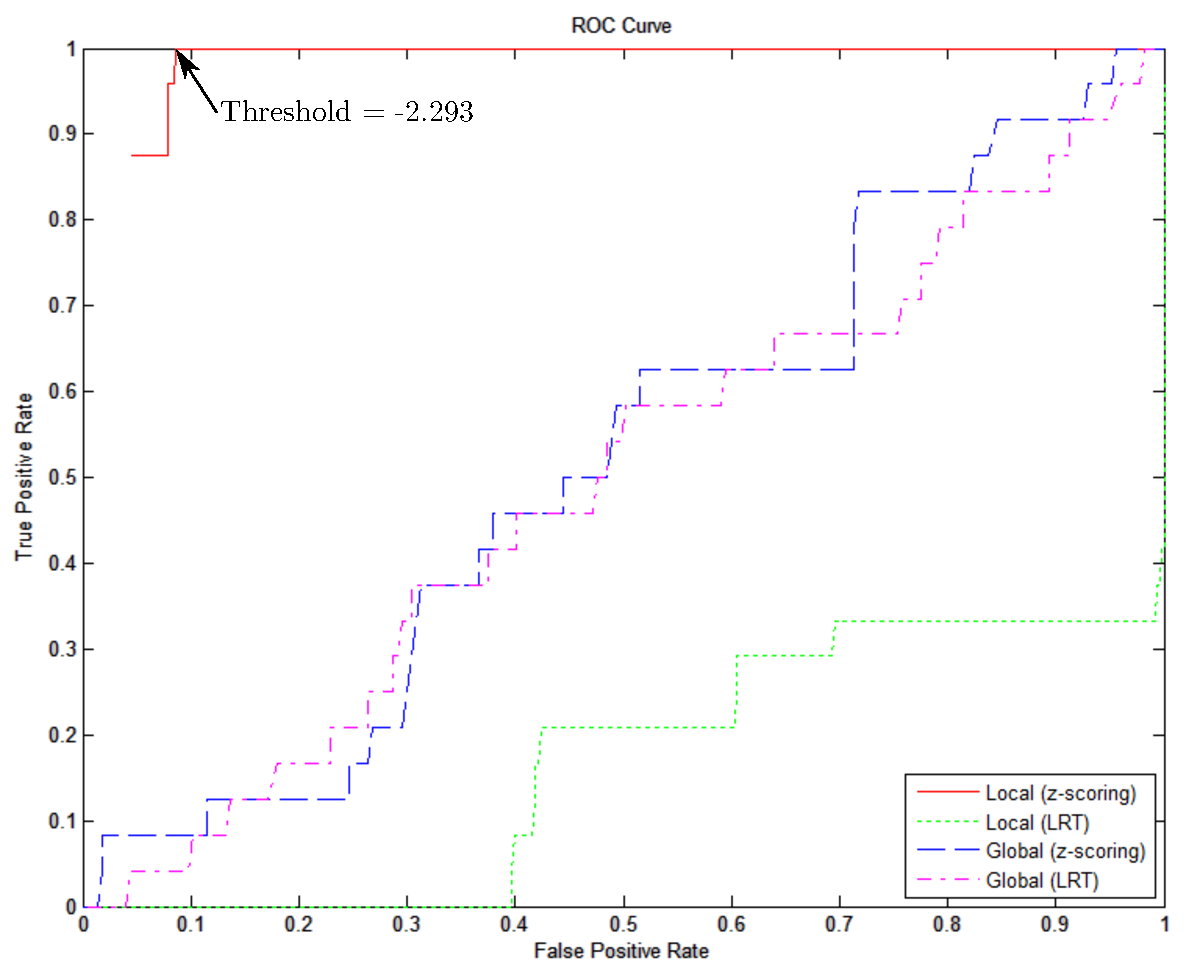
\includegraphics[width=2.8in]{figures/roc-ours-vs-global-results}
        \caption{Anomaly detection ROC
            curves. Solid red, dotted green, dashed blue, and dash-dot magenta
            lines represent ROCs for methods I, II, III, and IV,
            respectively.}
        \label{fig:roc-ours-vs-global-results}
    \end{figure}

\end{frame}

%--------------------------------------------------------------------

\begin{frame}
    \frametitle{Incremental Behavior Modeling}
    \framesubtitle{Experimental Results (cont.)}
    
    The ROC curves and FP rates show that our method clearly outperforms
    the other three methods, but there is also a surprising interaction.

    \bigskip

    For the global method, $z$-scored likelihood and LRT are equally
    effective, but for our local event based method, $z$-scoring is much
    more effective than the LRT.  
    
    \bigskip
    
    This may reflect that the LRT's use of a mixture model is less 
    appropriate for the local method than the global method.
    
\end{frame}

%--------------------------------------------------------------------

\begin{frame}
    \frametitle{Incremental Behavior Modeling}
    \framesubtitle{Experimental Results (cont.)}
    
    \begin{table}
        \centering
        \caption{Anomaly detection results for the local method with
            the $z$-scoring method and the likelihood ratio test, and the
            global method with the $z$-scoring method and likelihood ratio
            test.}
        \begin{tabular}{c|c|c|c|c|c|c}
            \hline Batch method & TP & FP & TN & FN & TPR & FPR \\ \hline \hline
            Local ($z$-scoring) & 24 & 42 & 444 & 0 & 1 & 0.086 \\ \hline
            Local (LRT) & 24 & 486 & 0 & 0 & 1 & 1 \\ \hline 
            Global ($z$-scoring) & 24 & 217 & 10 & 0 & 1 & 0.956 \\ \hline 
            Global (LRT) & 24 & 223 & 4 & 0 & 1 & 0.982 \\ \hline
        \end{tabular}
        \label{tab:hmm-based-detection-results}
    \end{table} 

\end{frame}

%--------------------------------------------------------------------

\begin{frame}
    \frametitle{Incremental Behavior Modeling}
    \framesubtitle{Experimental Results (cont.)}
    
    The reason that the local method is better than the global method
    (albeit when combined with $z$-scoring of the likelihood) is that 
    
    \begin{itemize}
        \item Many of the abnormal sequences in the test set tend to be 
            locally similar to the abnormal sequences in the bootstrap set 
            but globally different. 
        \item The local method treats concurrent but spatially separate
            local events as being independent, whereas the global method 
            attempts to construct a joint model over the entire scene. 
            The global method might be improved with a larger bootstrap set.
    \end{itemize}

\end{frame}

%--------------------------------------------------------------------

\begin{frame}
    \frametitle{Incremental Behavior Modeling}
    \framesubtitle{Experimental Results (cont.)}
    
    The log likelihood ratio test fails to detect completely new anomalous
    patterns when the pattern has a very low likelihood according to the
    abnormal model and the normal model but has a slightly higher
    likelihood according to the normal model. 
    
    \bigskip
    
    In order for the LRT test to
    detect such patterns, we need to adjust the LR threshold, causing
    higher false positives (increasing the number of false positives to
    about 30--40).  
    
    \bigskip
    
    Since our approach creates a new abnormal model for
    any low-likelihood observation, regardless of the relative likelihood,
    it does not suffer from this problem.
    
\end{frame}

%--------------------------------------------------------------------

\begin{frame}
    \frametitle{Incremental Behavior Modeling}
    \framesubtitle{Experimental Results (cont.)}
    
    We used the same settings and model configuration as in the batch 
    method experiments described previously.
   
    \bigskip

    Since we incorporate a completely new observation sequence at each 
    increment, the likelihood over all the sequences may increase or 
    decrease. 
    
    \bigskip
    
    In the current work, we reestimate $\mu_c$ and $\sigma_c$ after every 
    update by generating 1,000 new sample sequences.  The update process 
    could obviously be optimized.

\end{frame}

%--------------------------------------------------------------------

\begin{frame}
    \frametitle{Incremental Behavior Modeling}
    \framesubtitle{Experimental Results (cont.)}

    \begin{figure}
        \centering
        \subfloat[]{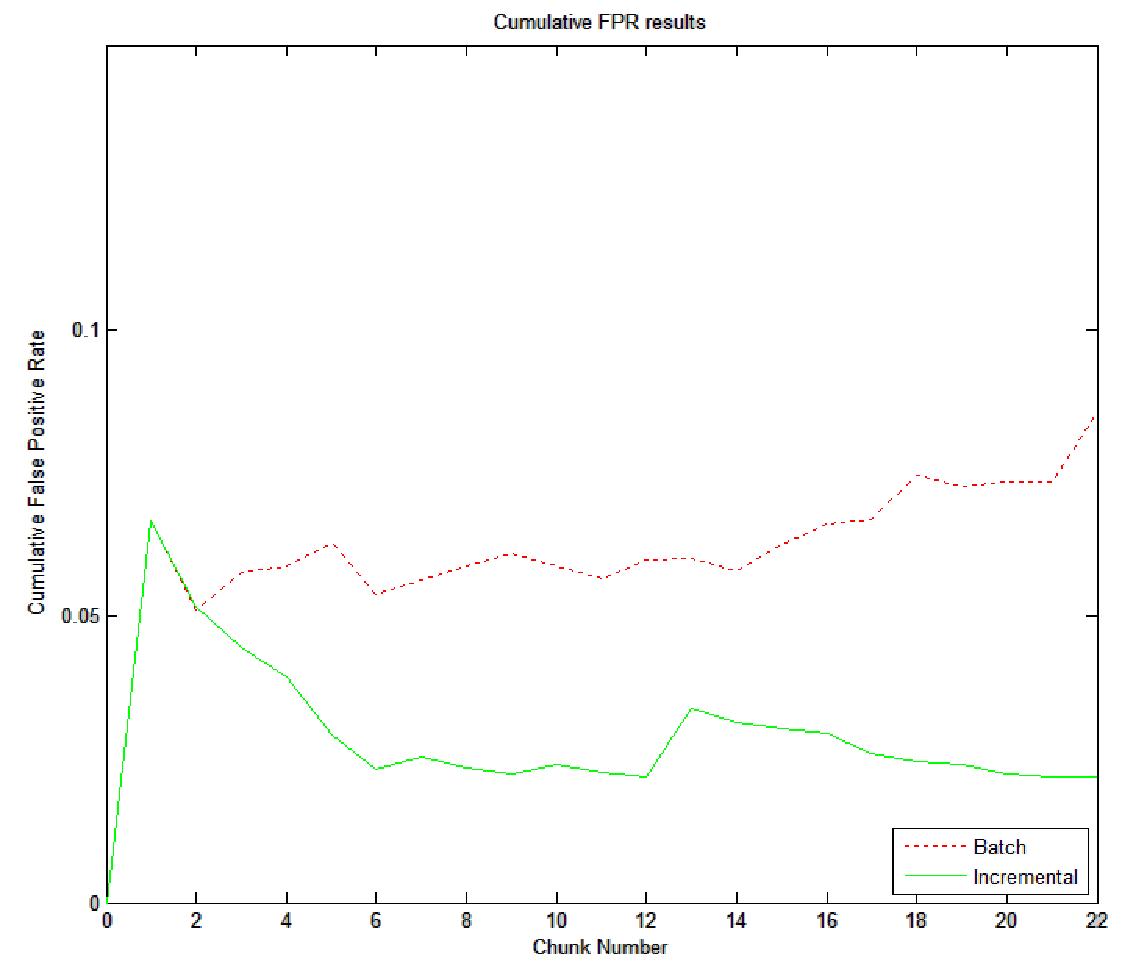
\includegraphics[width=2.2in]{figures/cFPR-chunk-results-5-trials}}
        \subfloat[]{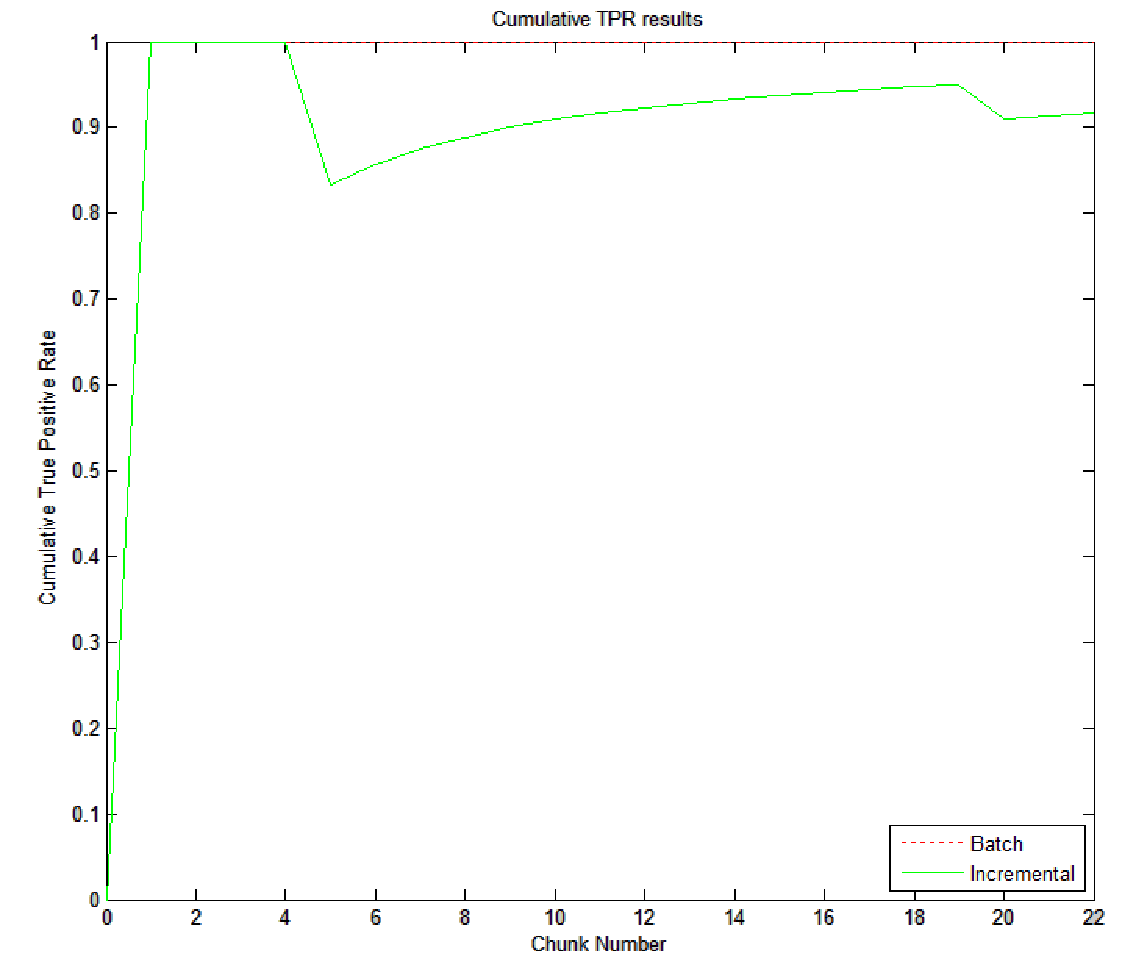
\includegraphics[width=2.2in]{figures/cTPR-chunk-results-5-trials}}
        \caption{Comparison of batch learning (dotted red line) and
            incremental learning (solid green line) over time.  (a) Cumulative
            false positive rates. (b) Cumulative true positive rates.  Each
            point is an average of the false positive or true positive rates
            over 5 trials.}
        \label{fig:chunking-results}
    \end{figure}

\end{frame}

%--------------------------------------------------------------------

\begin{frame}
    \frametitle{Incremental Behavior Modeling}
    \framesubtitle{Experimental Results (cont.)}

    \begin{table}
        \caption{Anomaly detection results on average for
            incremental HMM learning for our local method and the global
            method over 5 trials.}
            \centering
            \begin{tabular}{c|c|c|c|c|c|c}
                \hline
                Incremental method & TP & FP & TN & FN & TPR & FPR \\
                \hline \hline
                Local ($z$-scoring) & 21.8 & 9.8  & 476.2  & 2.2 & 0.91 & 0.022 \\ \hline
                Local (LRT) & 16 & 243.4 & 212.6 & 8 & 0.6664 & 0.564 \\ \hline
                Global ($z$-scoring)  & 3 & 13 & 214 & 21 & 0.125 & 0.057 \\ \hline
                Global (LRT)  & 18 & 184.4 & 42.6 & 6 & 0.75 & 0.813 \\ \hline
            \end{tabular}
        \label{tab:iml-detection-results}
    \end{table}

\end{frame}

%--------------------------------------------------------------------

\begin{frame}
    \frametitle{Incremental Behavior Modeling}
    \framesubtitle{Experimental Results (cont.)}

    Compared to the batch method, the
    incremental version of the proposed method (local method with
    $z$-scoring) obtains a nearly four-fold decrease in the false positive
    rate (2.2\% vs.\ 8.6\%) at the cost of a 9\% decrease in the hit rate.

    \bigskip
    
    To better enable comparison of the
    results for batch and incremental learning, we varied $\theta_z$ to
    obtain false positive rates at 100\% detection rates and to obtain
    equal error rates (EERs). 
    
    \bigskip
    
    The incremental method achieves a 3.7\%
    false alarm rate at a 100\% hit rate, compared to 8.6\% for the batch
    method.  It achieves an EER of 95.8\%, compared to 91.8\% for the
    batch method.

\end{frame}

%--------------------------------------------------------------------

\begin{frame}
    \frametitle{Incremental Behavior Modeling}
    \framesubtitle{Discussion}

    We have proposed an efficient method for bootstrapping 
    scene-specific anomalous human behavior detection systems that 
    incrementally learns behavior models \alert{without} requiring storage
    of large databases of training data. 
    
    \bigskip
    
    The method requires minimal involvement of a human operator; the only 
    required action is to label the 
    patterns in a small bootstrap set as normal or anomalous and
    then to label false positive alarms as normal when they occur.

\end{frame}

\fi

